
%============================================================================
\section{The Design of an Integrated Verification Environment}\label{sec:va:general-mechanisms}
%============================================================================

The \EVE integrated verification environment is built on top of the EiffelStudio IDE and supplements it with functionalities for verification.

%----------------------------------------------------------------------------
\subsection{Contracts}
%----------------------------------------------------------------------------

The choice of Eiffel as programming language ensures that we rely on formal specification elements embedded in the program text as \emph{contracts} (pre and postconditions, class invariants, and other annotations).
Since correctness is a relative notion (being dependent on a specification), every verification activity requires \emph{some form} of specification.
Empirical evidence suggests that formal specifications in the form of contracts are a good compromise between the rigor required by formal techniques and the kind of effort that practitioners are able, or willing, to provide \cite{CHALIN06,POLIKARPOVA09}.

Not all contracts must be written by programmers: the architecture of \EVE can accommodate components for \emph{specification inference} to help users write better and stronger contracts.
This particular property, however, is not emphasized in the present discussion, which focuses on the integration of static and dynamic analysis assuming some contracts are available.

%----------------------------------------------------------------------------
\subsection{Automation}
%----------------------------------------------------------------------------

A defining characteristic of the tools in \EVE is that they are automatic and can do most of the work without any explicit input from the user, assuming the presence of contracts which Eiffel  programmers are already used to provide.
In order to decouple the machinery of the individual verification tools and to filter out their output, \EVE relies on a blackboard architecture~\cite{HUNT02} shown in Figure~\ref{fig:blackboard}.

\begin{figure}[!ht]%
\centering
\includegraphics[width=0.8\columnwidth,page=4]{images/drawings.pdf}
\caption{\EVE's blackboard architecture (gray boxes currently not implemented).}%
\label{fig:blackboard}%
\end{figure}


A \emph{controller} is responsible for triggering the various tools when appropriate, invisibly to the users. 
The controller bases its decisions on what the user is currently doing, which resources are available, and the results of previous verification attempts.
The latter are collected in a \emph{data pool} where every verification tool stores the results of its runs.
Users do not directly read the output of individual tools in the data pool.
Instead, the controller summarizes the output data and displays individual tool results only upon explicit user request.

A major design decision of \EVE was to make the verification mechanisms as unobtrusive as possible.
Users can continue using the IDE and their preferred software development process as before; the verification techniques are an additional benefit, available on demand and compatible with the rest of the IDE's tools.
In the same way that type checking adds a new level of help on top of the more elementary mechanisms of syntax error checking, \EVE provides reports from proofs and tests on top of the simple verification techniques provided by type checking.

%----------------------------------------------------------------------------
\subsection{Interaction with the user}
%----------------------------------------------------------------------------

Users have currently two ways to control the verification: (1) manually launch the tools or (2) use the fully automatic controller.
When using manual mode, the user chooses which tool to run on a specific class.
The tool will run in the background and the result will be added to the data pool when available, which will also automatically update the summary display.
Automatic mode has only the limited option of being enabled or disabled.
Even when enabled, verification never interferes with the more traditional development activities: \EVE works in the background on the latest compiled version of the system, and displays a summary of the verification results through an interface similar to that used to signal syntax or type errors in standard IDEs (Figure~\ref{fig:motivating-screenshot}).
At any time, the user can browse through the \emph{result list}, which links back to the parts of the program relevant for each message, and decide to revise parts of the implementation or specification according to the suggestions provided by \EVE.

Every entry in the result list has a \emph{score}: a quantitative estimate of the correctness or incorrectness of the associated entry, based on the evidence gathered so far by running the various tools.
The score varies over the real interval $[-1,1]$ (In the user interface the scale is, for more readability, $-100$ to $+100$, with rounding to the closest integer). 
A positive score indicates that the evidence in favor of correctness prevails, whereas a negative score characterizes evidence against correctness. The absolute value of the score indicates the level confidence: $1$ is conclusive evidence of correctness (for example a successful correctness proof), $-1$ is conclusive evidence of incorrectness (for example a failing test case), and $0$ denotes lack of evidence either way. Figure~\ref{fig:motivating-screenshot} shows an example of report with scores and stripes colored accordingly. Section~\ref{sec:va:scores} discusses how the score is computed for the verification tools currently integrated in \EVE.


%----------------------------------------------------------------------------
\subsection{Modularity and granularity}
%----------------------------------------------------------------------------

Object-oriented design emphasizes modularity, from which verification can also benefit.
While the level of granularity achievable by an integrated verification environment ultimately depends on the level of granularity provided by the tools it integrates, \EVE orients verification at the two basic levels of encapsulation provided by the object-oriented model: \emph{classes} and \emph{routines} within a class.
\EVE associates \emph{correctness scores} with items at both levels. Additional information may be attached to a correctness score, such as the line where a contract violation occurs in a test run, or the abstract domain used in an abstract interpretation analysis.
For large systems, it is also useful to have scores for highest levels of abstraction, such as groups of classes or entire libraries, but in the present discussion we limit ourselves to routine and class levels.

The scores from multiple sources of data at the same level are combined with weighted averages, and define the correctness scores at coarser levels.  
For example, every tool $t$ tries to verify a routine $r$ in class $C$ and reports a correctness score $s_r^C(t) \in [-1,1]$.
The cumulative score for the routine $r$ is then computed as the normalized weighted average:
\begin{equation}
s_r^C \ =\ \frac{1}{\sum_{t \in T} w_r^C(t)} \cdot \sum_{t \in T} w_r^C(t)s_r^C(t)
\label{eq:routine}
\end{equation}
where $w_r^C(t) \in \mathbb{R}_{\geq 0}$ denotes the weight (or \emph{confidence}) of the tool $t$ on routine $r$.
A similar expression computes the cumulative score $s^C$ for a class $C$ from the scores $s_r^C$ of its routines and their weights $w_r^C$:
\begin{equation}
s^C \ =\ \frac{1}{\sum_{r \in R} w_r^C} \cdot \sum_{r \in R} w_r^Cs_r^C
\label{eq:class}
\end{equation}

The weights take various peculiarities into account:
\begin{itemize}
\item
A tool may not be able to handle certain constructs: its confidence should be scaled accordingly.
For example, a tool unable to handle exceptions appropriately has its score reduced whenever it analyzes a routine which may raise exceptions.

\item
The results of a tool may be critical for the correctness of a certain routine.
For example, a quality standard may require that every public routine be tested for at least one hour without hitting a bug; correspondingly, the weight $w_r^C(t)$ for public routines $r$ would be high for testing tools and low (possibly even zero) for every other tool.

\item
The correctness of a routine may be critical for a class; then the routine score should have a higher weight in determining the class cumulative score.

\item
More generally, the weight may reflect suitable \emph{metrics} that estimate the criticality of a routine according to factors such as the complexity of its implementation or specification, whether it is part of the interface of public, and the number of references to it in clients or within the containing class.

\item
Similar metrics are applicable at other levels of granularity, for example to weigh the criticality of a class within the system.

\end{itemize}

\EVE provides default values for all the weights (Section~\ref{sec:va:scores}), but users can override them to take relevant domain knowledge into account.





%----------------------------------------------------------------------------
\subsection{Extensibility}
%----------------------------------------------------------------------------

The architecture of \EVE is \emph{extensible} to include more tools of heterogeneous nature.
The user interface will stay the same, with the blackboard controller being responsible for managing the tools optimally and only reporting the results through the summary scores described above.

The architecture can also accommodate tools that, while not targeted to verification in a strict sense, enhance the user experience.
For example, tools for assertion inference---such as AutoInfer \cite{WEI11} developed by other members of my group---can complement user-provided contracts and improve the performance of approaches that depend on contracts.
The controller can activate assertion inference when the verification machinery performs poorly and when metrics suggest that the code is lacking sufficient specifications.
The assertion inference tools themselves may sometimes re-use the results of other tools; for example AutoInfer relies on the test cases generated by \AutoTest.
Finally, \EVE can show the inferred assertions in the form of suggestions, in connection with the results of other verification activities.
For example, it could display an inferred loop invariant with the report of a failed proof attempt, and suggest that the invariant can make the correctness proof succeed if added to the specification.
The current implementation of \EVE does not integrate such suggestions mechanisms yet. %, but the architecture is designed with these extensions in mind.


